\documentclass[aspectratio=169,11pt]{beamer}
\usepackage[T2A,T1]{fontenc}
\usepackage[utf8]{inputenc}
\usepackage[english,russian]{babel}
\usepackage{lmodern}
\usepackage{graphicx}
\usepackage{booktabs}
\usepackage{amsmath,amssymb}
\usepackage{xcolor}

\graphicspath{
    {../results/slide_figs/}
    {../results/report_figs/}
    {results/slide_figs/}
    {results/report_figs/}
}

\usetheme{default}
\usecolortheme{whale}
\setbeamertemplate{navigation symbols}{}
\setbeamertemplate{footline}[frame number]
\setbeamercolor{title}{fg=structure!80!black}
\setbeamerfont{frametitle}{size=\large,series=\bfseries}
\setbeamerfont{title}{size=\Large,series=\bfseries}
\setbeamertemplate{itemize item}{\color{structure}\textbullet}

\setbeameroption{show notes}
\setbeamertemplate{note page}[plain]

\title{0--k BFS}
\subtitle{Кратчайшие пути с ограниченными целыми весами -- C++17}
\author{Артёмов Макар \and Марк Шкут}
\institute{Сколтех, Алгоритмы 2026}
\date{21 мая 2026}

\begin{document}

% ------------------------------------------------------------- 1: TITLE
\begin{frame}
  \titlepage
\end{frame}
\note{
\textbf{Открывающая фраза.}\\[0.4em]
Проект: 0--k BFS для задачи кратчайших путей с ограниченными целыми
весами на C++17. Совместная работа с Марком. Цель доклада: объяснить
семейство алгоритмов, показать, почему оно обгоняет Дейкстру на графах
с малыми целыми весами, и представить наши замеры вплоть до
$V = 9 \cdot 10^8$. Длительность: около 15 минут плюс вопросы.
}

% ------------------------------------------------------------- 2: PROBLEM
\begin{frame}{Задача}
\begin{itemize}
  \item Кратчайшие пути из одной вершины в графе $G=(V,E,w)$
  \item Веса принимают значения из $\{0,1,\dots,k\}$ при небольшом известном $k$
  \item Цель: $V$ приближается к $10^9$ на одной рабочей станции
\end{itemize}
\vspace{0.6em}
\textbf{Где встречается:} планирование путей на сетках, слоистые графы,
сведения к 2-SAT, транспортные сети с несколькими уровнями стоимости.
\end{frame}
\note{
\textbf{Чётко формулируем задачу.}\\
Нам нужны все расстояния от одной вершины-источника. Особенность в том,
что веса -- неотрицательные целые числа, ограниченные сверху небольшим
$k$. Это ограничение не искусственное: оно постоянно встречается на
сетках, в слоистых DAG, в задачах олимпиадного программирования.
Алгоритмически интересно, потому что для маленьких целых весов мы
можем превзойти классическую Дейкстру $O((V+E)\log V)$.\\
\textbf{Зачем целиться в $V \to 10^9$:} это форсирующее условие
дизайна -- именно оно потребует неявного графа и 32-битных расстояний,
о которых будет дальше.
}

% ------------------------------------------------------------- 3: BASELINE
\begin{frame}{Базовый алгоритм: Дейкстра}
\begin{itemize}
  \item \texttt{std::priority\_queue<pair<Distance,Vertex>>}, ленивое decrease-key
  \item $O((V+E)\log V)$ времени, $O(V+E)$ памяти
  \item Работает для любых неотрицательных вещественных весов
\end{itemize}
\vspace{0.4em}
Множитель $\log V$ -- это цена кучи. \emph{Если веса малые целые, можем
ли мы заменить кучу на что-то более дешёвое?}
\end{frame}
\note{
\textbf{Определяем Дейкстру как baseline.}\\
Это классический алгоритм, который все знают. Реализация прямая: куча
пар (расстояние, вершина) с ленивым decrease-key (повторно кладём, на
поп пропускаем устаревшие записи). Множитель $\log V$ платится в каждой
успешной релаксации. Вся идея 0--k BFS в том, что при маленьких целых
весах куча вообще не нужна.\\[0.3em]
\textit{Пауза для вопроса на слайде -- это мотивирует следующий слайд.}
}

% ------------------------------------------------------------- 4: 0-1 BFS
\begin{frame}{Идея: 0--1 BFS}
Веса 0 или 1. Заменяем очередь с приоритетом на \textbf{deque}:
\begin{itemize}
  \item ребро веса 0 $\to$ \texttt{push\_front}
  \item ребро веса 1 $\to$ \texttt{push\_back}
\end{itemize}
\vspace{0.3em}
Дек всегда отсортирован по расстоянию, состоит из двух непрерывных слоёв.
\begin{center}
\textbf{Сложность:}\quad $O(V+E)$\qquad
\textbf{Память:}\quad $O(V)$
\end{center}
\end{frame}
\note{
\textbf{Педагогический центр, часть~1.}\\
Идея простая. В любом BFS у нас есть ``текущий слой'' и ``следующий
слой''. При весах 0/1 ребро веса 0 оставляет нас в текущем слое
(перёд дека, обрабатывается сразу), а ребро веса 1 переводит в
следующий (хвост дека). Дек всё время упорядочен по расстоянию и
содержит максимум два различных значения.\\
Важная деталь по сравнению с обычным BFS: вершина может быть открыта
несколько раз до того, как её расстояние станет окончательным. Поэтому
при каждой релаксации проверяем не ``посещена/нет'', а
\emph{dist[v] + w(v,u) < dist[u]}.
}

% ------------------------------------------------------------- 5: 0-k BFS
\begin{frame}{Обобщение: 0--k BFS}
Веса $\{0,1,\dots,k\}$. Используем \textbf{$k+1$ FIFO-очередь}, индексируем
их по $\mathrm{dist}[v] \bmod (k+1)$.
\begin{itemize}
  \item ``Активный'' бакет $\mathrm{cur}$ движется вперёд
  \item Релаксация кладёт $v$ в бакет $(d_{\text{new}}) \bmod (k+1)$
  \item Устаревшие записи пропускаются при поп
\end{itemize}
\begin{center}
\textbf{Сложность:}\quad $O(kV+E)$\qquad
\textbf{Память:}\quad $O(k+E)$ на очереди
\end{center}
\end{frame}
\note{
\textbf{Педагогический центр, часть~2.}\\
Обобщаем: при весах до $k$ релаксация может продвинуть вершину на
расстояние ещё $+k$. Значит, в любой момент живых ``слоёв''
расстояний не больше $k+1$. Заводим $k+1$ FIFO-очередей и индексируем
по $\text{dist} \bmod (k+1)$ -- кольцевой буфер бакетов.\\
Отсюда и название ``circular FIFO queues''. Указатель \texttt{cur}
обходит их; когда текущий бакет опустеет, переходим к следующему. Если
вершину переоткрыли с меньшим расстоянием, она попадает в другой бакет,
а исходная запись становится устаревшей и пропускается при поп.
}

% ------------------------------------------------------------- 6: VISUAL
\begin{frame}{Как это выглядит}
\centering
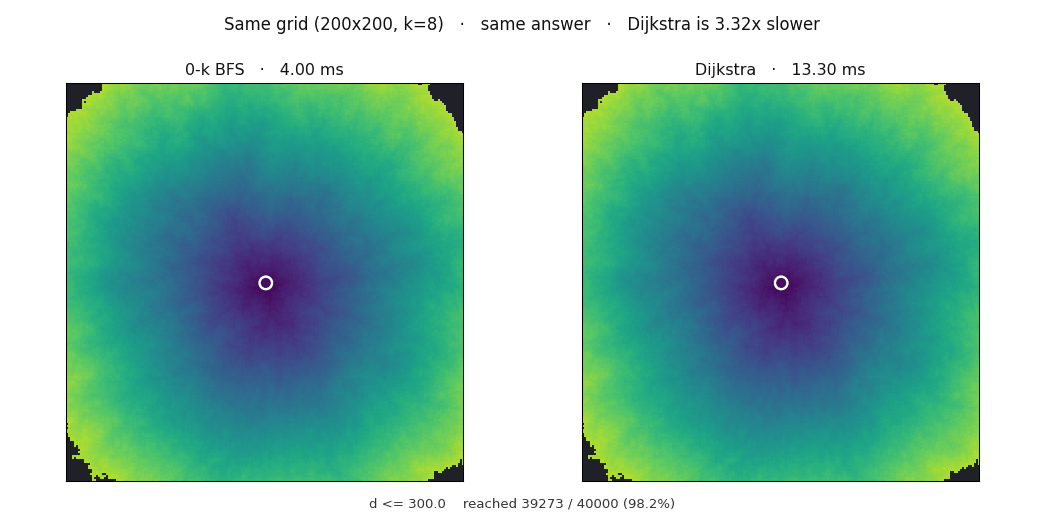
\includegraphics[width=0.86\linewidth]{compare_still.png}
\\[0.2em]
\footnotesize Одна и та же сетка 200$\times$200, $k=8$. Один и тот же ответ.
0--k BFS \textbf{4.00 мс}, Дейкстра \textbf{13.30 мс} -- в 3.32$\times$ медленнее.
\end{frame}
\note{
\textbf{Показываем сравнительную анимацию (или этот кадр).}\\
``Оба алгоритма выдают одинаковое поле расстояний. Левая панель завершает
волну за 4 миллисекунды, правая за 13.3 -- разница вся в том, что
каждая релаксация в Дейкстре платит логарифмический фактор кучи.
Анимация в репозитории запускает оба алгоритма синхронно, а в
заголовках выписаны реальные времена.''\\
\textbf{Тезис:} визуализация -- тоже часть проекта; именно через неё мы
сами проверяли алгоритм, прежде чем измерять.
}

% ------------------------------------------------------------- 7: QUEUES
\begin{frame}{Под капотом}
\centering
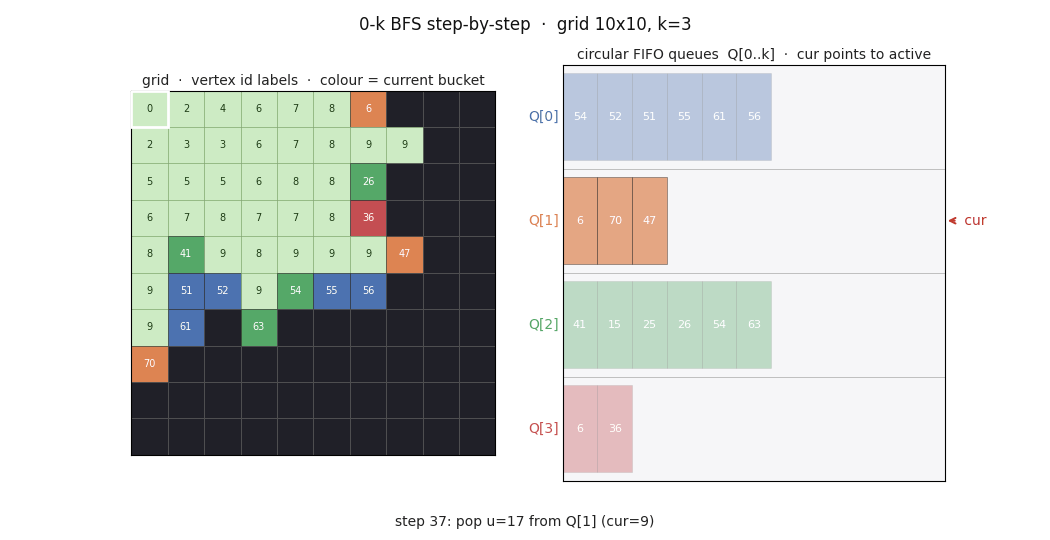
\includegraphics[width=0.85\linewidth]{queues_still.png}
\\[0.2em]
\footnotesize Пошагово на маленькой сетке $10\times10$, $k=3$.\,
Каждая строка справа -- одна очередь $Q[0]\dots Q[3]$;\,
\textcolor{red}{\textbf{cur}} указывает на активный бакет.
\end{frame}
\note{
\textbf{Закрепляем структуру данных.}\\
Справа видны реальные четыре очереди $Q[0]$\,--\,$Q[3]$ с их текущим
содержимым (числа -- идентификаторы вершин). Слева сетка, цвета клеток
показывают, в каком бакете сейчас лежит вершина. На этом кадре
\texttt{cur} указывает на $Q[1]$.\\
Анимация -- скрипт \texttt{viz/animate\_queues.py}, который потребляет
пошаговый журнал, выгружаемый инструментированным алгоритмом на C++
(\texttt{include/zkbfs/bfs0k\_trace.hpp}). Именно эта картинка делает
алгоритм \emph{обучаемым}: вся суть в очередях.
}

% ------------------------------------------------------------- 8: SCALE
\begin{frame}{Дизайн под V $\to 10^9$}
\begin{itemize}
  \item Явный CSR при $V=10^9$ стоит $\sim$20 ГБ только на рёбра -- \emph{невозможно}
  \item \texttt{GridGraph}: неявная 4-связная сетка, $O(1)$ на соседа, рёбра не хранятся
  \item \texttt{Distance = uint32\_t}: уменьшает доминирующий массив вдвое (4 ГБ вместо 8 ГБ)
  \item Допустимо, пока $k \cdot V < 2^{32}$
\end{itemize}
\end{frame}
\note{
\textbf{Защищаем дизайнерские решения, благодаря которым возможен большой
запуск.}\\
Бэкендов два. Универсальный \texttt{GraphCSR} упирается в потолок около
$V \approx 10^8$ из-за памяти. \texttt{GridGraph} неявный: рёбра не
храним, вычисляем по запросу. Это плюс 32-битное расстояние --
именно так мы фактически прогнали $V = 9 \cdot 10^8$ при 14 ГБ
свободной RAM.\\
Честная оговорка: 32-битное расстояние работает не всегда. Требование:
$k \cdot V < 2^{32}$. Для наших параметров это выполнено, плюс есть
64-битный fallback через флаг компиляции.
}

% ------------------------------------------------------------- 9: RESULTS
\begin{frame}{Результаты, сетка, один поток}
\centering
\small
\begin{tabular}{rrrrr@{}r}
\toprule
$V$            & $k$ & Дейкстра & 0--k BFS & 0--1 BFS & ускорение \\ \midrule
$10^6$         & 1   & 0.180 с  & 0.039 с  & 0.070 с  & 4.6$\times$ \\
$10^7$         & 1   & 1.98 с   & 0.493 с  & 0.355 с  & 5.6$\times$ \\
$10^8$         & 1   & 60.3 с   & 28.4 с   & 5.44 с   & \textbf{11.1}$\times$ \\
$4.84\cdot 10^8$ & 4 & 432.9 с  & 451.4 с  & ---      & 0.96$\times$ (пам.) \\
\textbf{$9\cdot 10^8$} & 1 & \textbf{619.9 с} & --- & \textbf{121.2 с} & \textbf{5.12}$\times$ \\
\bottomrule
\end{tabular}
\\[0.6em]
Оба алгоритма дают \emph{побайтово совпадающие} контрольные суммы
расстояний на каждом инстансе.
\end{frame}
\note{
\textbf{Проходим таблицу сверху вниз.}\\
Уже при $V=10^6$ получаем ускорение в 4--5$\times$. При $V=10^8$ и
$k=1$ deque-вариант 0--1 BFS в 11$\times$ быстрее Дейкстры. Строка
$V \approx 5 \cdot 10^8$ интересна -- разрыв схлопывается, оба алгоритма
становятся memory-bandwidth bound. Внизу заголовочный результат: на 900
миллионах вершин 0--1 BFS заканчивает за две минуты, Дейкстра -- за
десять.\\
Важно: все контрольные суммы совпадают; корректность проверена на 19
различных инстансах в свипе, ноль расхождений.
}

% ------------------------------------------------------------- 10: PLOT
\begin{frame}{Масштабирование}
\centering
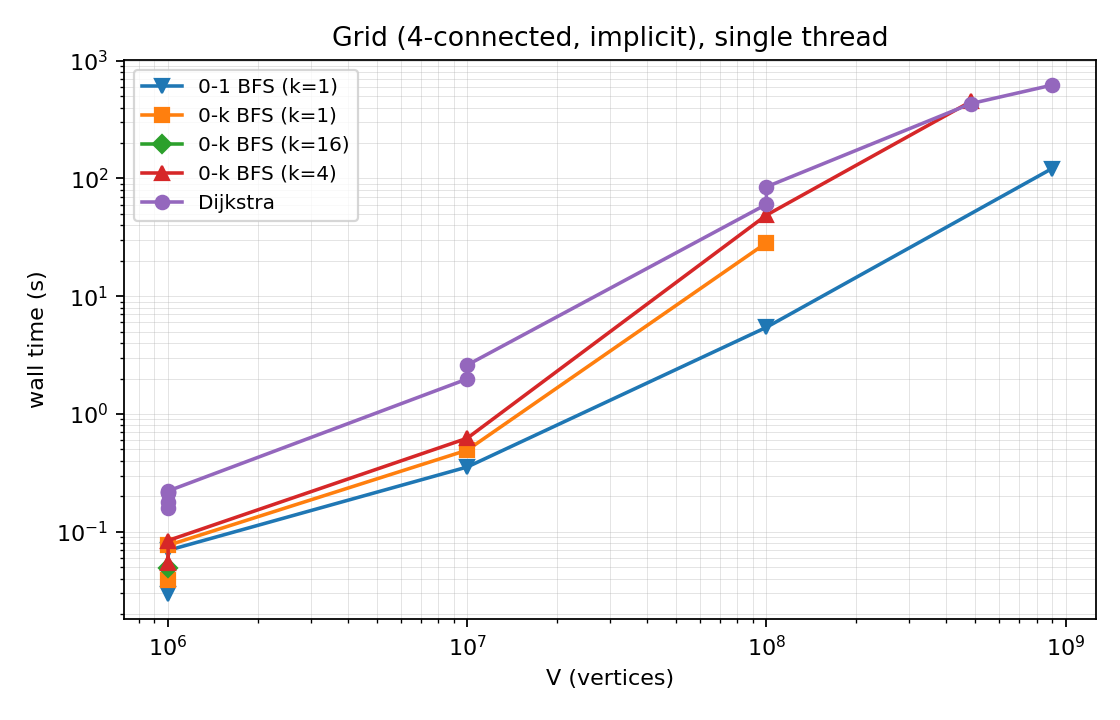
\includegraphics[width=0.72\linewidth]{grid_scaling.png}
\end{frame}
\note{
\textbf{Разбираем график.}\\
Обе оси логарифмические. Пять серий: Дейкстра вверху, варианты BFS идут
параллельно ниже. Постоянный вертикальный зазор в логарифмической шкале
соответствует примерно постоянному мультипликативному ускорению. При
$V=10^8$ и выше линии начинают сходиться -- входим в memory-bound
режим. Самая нижняя линия везде -- deque-вариант 0--1 BFS, наиболее
чистая реализация в семействе.
}

% ------------------------------------------------------------- 11: LIMITS
\begin{frame}{Ограничения}
\begin{itemize}
  \item Ускорение уменьшается с ростом $k$ -- исчезает при $k = \omega(\log V)$
  \item При $V \gtrsim 5 \cdot 10^8$ оба алгоритма упираются в пропускную способность памяти
  \item Двухочередной $bfs\_0k$ медленнее однодекового $bfs\_01$ при большом $V$ (аллокатор) -- $k+1$ очередь = $k+1$ аллокатор
  \item Требуются неотрицательные целые веса с известным малым $k$
\end{itemize}
\end{frame}
\note{
\textbf{Честно про границы применимости.}\\
Во-первых: это выигрыш по константе, не по асимптотике. Как только $k$
сравним с $\log V$, Дейкстра не хуже.\\
Во-вторых: на гигантских $V$ всё упирается в память. Мы видели, как
0--k BFS приходит к паритету с Дейкстрой при $V \approx 5 \cdot 10^8$.
Реализация имеет огромное значение: содержать $k+1$ отдельный
аллокатор очередей дороже для кэша и аллокатора, чем один deque --
поэтому 0--1 BFS у нас продолжает выигрывать при $V = 9 \cdot 10^8$, а
общий 0--k BFS на этом масштабе уже нет.\\
В-третьих: это не замена Дейкстре в общем случае. Для вещественных
весов или неизвестного бакета -- использовать Дейкстру.
}

% ------------------------------------------------------------- 12: NEXT
\begin{frame}{Дальнейшие шаги}
\begin{itemize}
  \item Индексная $d$-арная куча для Дейкстры (честный decrease-key)
  \item Кусочный кольцевой FIFO для \texttt{bfs\_0k} (закрыть разрыв с 0--1 BFS)
  \item Загрузчик дорожной сети (DIMACS USA, веса квантуем до $k=8$)
  \item Стретч: $\Delta$-stepping для параллельного контекста
\end{itemize}
\end{frame}
\note{
\textbf{Куда движемся.}\\
Четыре пункта. Первые два -- доводка реализации: настоящая куча с
decrease-key как более честный baseline и кусочная очередь, чтобы
догнать cache-поведение дека. Третий -- выйти из зоны синтетических
графов на реальную дорожную сеть. Четвёртый -- $\Delta$-stepping, это
канонический параллельный родственник 0--k BFS; полезно иметь хотя бы
для контекста, даже если параллелизм мы не разгоняем всерьёз.
}

% ------------------------------------------------------------- 13: END
\begin{frame}{Спасибо}
\begin{itemize}
  \item Код, отчёт, графики: \texttt{github.com/artemovmak/EffectiveAlgorithms}
  \item Отчёт по Этапу~1: \texttt{stage1\_report.pdf}
\end{itemize}
\vspace{0.6em}
Вопросы?
\end{frame}
\note{
\textbf{Закрытие.}\\
Всё -- код, LaTeX-отчёт, анимации, воспроизводимые скрипты сборки --
лежит в репозитории на GitHub. Переходим к вопросам. Вероятные
вопросы:\\[0.2em]
\textit{В:} ``Почему 0--1 BFS быстрее 0--k BFS при $k=1$?'' -- накладные
расходы аллокатора двух \texttt{std::queue} против одного
\texttt{std::deque}.\\
\textit{В:} ``Как проверяли корректность на запуске с миллиардом вершин?''
-- контрольные суммы расстояний совпадают с Дейкстрой побайтово; поэлементное
сравнение не нужно, сумма уже фиксирует массив.\\
\textit{В:} ``А параллелизм?'' -- весь Этап~1 в один поток;
$\Delta$-stepping -- запланированный стретч-таргет на Неделю~2.
}

\end{document}
